\clearpage
\section{Detailed Description of the Work Plan}

% AP mit Arbeitsumfängen Darstellung Voraussetzungen, Lösungswegen, Entscheidungspunkten, Umgang mit möglichen Risiken
% In jedem Fall zu betrachten: Wie wird der Problemlösungsraum eingeschränkt? Woran wird der Projekterfolg gemessen? Risikomanagement (wissenschaftlich/technisch)
% Bei ergebnisoffenem Prozess: klare Definition der Arbeitspakete und Ziele, Wie wird das Projektergebnis definiert? Wie kommt es zu Entscheidungspunkten?

Im Folgenden werden die geplanten Arbeitspakete und Meilensteine (\Cref{subsec:ap}), Zeit- und Ressourcenplanung (\Cref{subsec:zeitplan}) und Finanzplanung (\Cref{sec:finanz}) im Detail beschrieben.

\subsection{Work packages and milestones}
\label{subsec:ap}

\begin{figure}
    \centering
    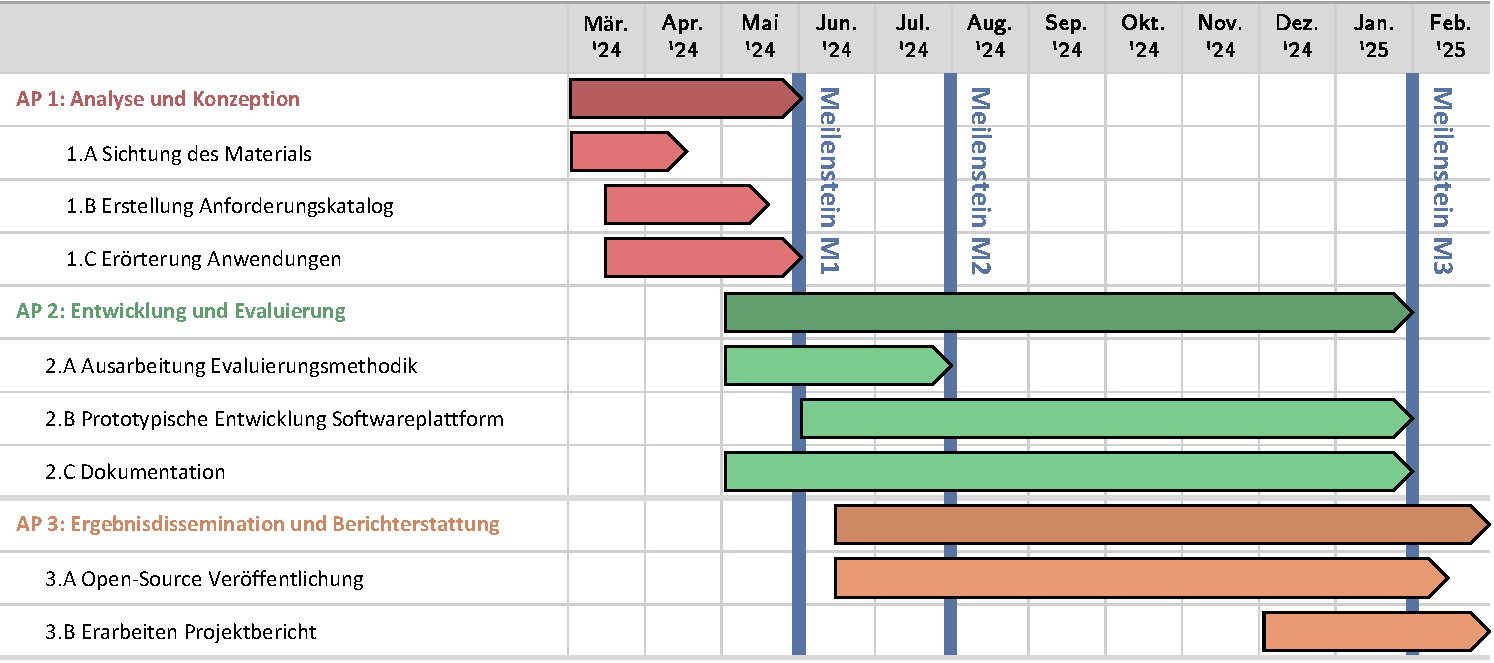
\includegraphics[width=\linewidth]{./graphs/gantt.pdf}
    \caption{Zeitplan des Projekts SPENCER.}
    \label{fig:gantt}
\end{figure}

Das Projekt SPENCER ist in die drei Phasen `Analyse und Konzeption', `Entwicklung und Evaluierung' und `Ergebnisdissemination und Berichterstattung' unterteilt.
Der Zeitplan der Arbeitspaketbearbeitung findet sich in \cref{fig:gantt}.

\subsubsection{AP1: ...}
\label{subsec:ap:1}

In der Analyse- und Konzeptionsphase liegt der Fokus auf einer umfassenden Untersuchung aktueller Publikationen wie Studien, Patente und Forschungsberichte sowie der Analyse technologischer Entwicklungen und wirtschaftlicher Rahmenbedingungen (Punkt 1.A).
Durch diese systematische Sichtung sollen fundierte Erkenntnisse gewonnen werden, die als Grundlage für die weitere Ausarbeitung des Projekts dienen.

Die enge Zusammenarbeit mit dem Industriepartner ermöglicht es, den Rahmen, die Grundlagen und die Qualitätsdimensionen des Projekts zu definieren.
Hierbei werden sowohl funktionale als auch nicht-funktionale Ziele identifiziert und in einem präzisen Anforderungskatalog festgehalten (Punkt 1.B).
Dieser Katalog dient als Leitfaden für die nachfolgenden Entwicklungs- und Evaluierungsphasen des Projekts.

Ein besonderes Augenmerk liegt dabei auf möglichen Anwendungen aus Domänen, die von Edge-Computing profitieren können (Punkt 1.C).
Die Identifikation und Betrachtung dieser Anwendungsfelder für die Bereitstellung global verteilter Software trägt dazu bei, zukünftige Entwicklungen und Chancen im Bereich des Edge-Computing zu antizipieren.

Als entscheidenden Meilenstein des ersten Arbeitspakets ist geplant, am Ende eine umfassende Grundlagenstudie zum Ist-Zustand vorzulegen (Meilenstein M1).
Diese Studie wird nicht nur einen detaillierten Anforderungskatalog umfassen, sondern auch eine tiefgehende Analyse aktueller Grundlagen und Entwicklungen im Bereich des global verteilten Edge-Computing bieten.
Die Ausarbeitung wird zudem eine präzise Auswahl von exemplarischen Anwendungsfeldern einschließen.

Die Grundlagenstudie wird als ein strategisches Dokument fungieren, das nicht nur den aktuellen Stand des Wissens und der Anforderungen widerspiegelt, sondern auch als Leitfaden für die nächsten Phasen des Projekts dient.
Durch die klare Definition von Rahmen, Qualitätsdimensionen und konkreten Zielen legt die Studie den Grundstein für eine effektive und zielgerichtete Umsetzung des Projekts.
Ihr Abschluss markiert somit nicht nur das Ende der Analyse- und Konzeptionsphase, sondern gleichzeitig den Startpunkt für die aufbauenden Schritte in der Entwicklungs- und Evaluierungsphase.

\subsubsection{AP2: ...}
\label{subsec:ap:2}

In der Phase der "Entwicklung und Evaluierung" erfolgt zunächst die gezielte Auswahl von drei Softwareanwendungen, innerhalb derer die Erfüllung der zuvor definierten Anforderungen aus Anwendungsperspektive intensiv untersucht werden kann.
Dies unterliegt dem Ansatz eines Test-Driven-Development-Prozess, der sicherstellt, dass die im Anforderungskatalog festgelegten Anforderungen systematisch in Evaluierungsmethoden umgesetzt werden, die während des Entwicklungsprozesses kontinuierlich Anwendung finden.
Hierzu gehören beispielsweise Tests für funktionale Aspekte sowie Performance-Benchmarks für nicht-funktionale Anforderungen (Punkt 2.A).
Die entwickelteten wiederverwendbaren Evaluationsmethodiken und -Umgebungen stellen somit den zweiten Meilenstein des Projekts dar (Meilenstein M2).
Sie bilden nicht nur die Grundlage für die darauf folgende Implementierung und Integration, sondern ermöglichen auch eine fundierte Evaluation und potenzielle Anpassung der entwickelten Lösung im Hinblick auf die ursprünglichen Anforderungen.

Durch eine kontinuierliche und strenge Anwendung dieser Evaluierungsmethoden an Prototypen wird so anschließend agil eine Serverless Edge-Computing Plattform entwickelt.
Diese Prototypenentwicklung orientiert sich an bestehenden Open-Source Software-Plattformen, die iterativ weiterentwickelt werden, um schließlich in einem finalen Software-Prototypen zu konvergieren (Punkt 2.B).
Die Entwicklung dieses Software-Prototypen umfasst die Entwicklung zweier Hauptkomponenten:
Erstens wird eine Serverless-Laufzeitumgebung entwickelt, die verschiedene Anwendungsdienste parallel aber isoliert auf begrenzten Resourcen ausführen kann und in der Lage ist, Resourcen schnell zwischen Diensten auszutauschen um Elastizität sicherzustellen.
Zweitens wird parallel aber in enger Absprache ein Subsystem zur Migration von Anwendungsdienstinstanzen und Dienstzustandsdaten entwickelt, um einen Transfer von Diensten entgegen der Mobilität der unterliegenden Satelliten-Infrastruktur zu gewährleisten.
Der Software-Prototyp, der die definierten Anforderungen erfüllt, stellt damit den dritten Meilenstein des Projekts dar (Meilenstein M3).

Die erfolgreiche Umsetzung dieses Entwicklungsprozesses erfordert zudem die Erstellung einer detaillierten technischen Dokumentation (Punkt 2.C).
Diese Dokumentation bildet nicht nur die Grundlage für die interne Weiterentwicklung der Plattform, sondern stellt auch sicher, dass das erarbeitete Wissen und die Funktionsweise der entwickelten Software auch über das Ende des Projekts hinaus transparent und nachvollziehbar sind.

\subsubsection{AP3: ...}
\label{subsec:ap:3}

In der Phase der "Ergebnisdissemination und Berichterstattung" stehen zwei entscheidende Aktivitäten im Mittelpunkt:
Zum einen erfolgt die Open-Source Veröffentlichung der entwickelten Softwarelösung (Punkt 3.A).
Dies ermöglicht anderen Fachleuten und Organisationen, von den erzielten Erkenntnissen und der entwickelten Serverless Edge-Computing Plattform zu profitieren.
Die Open-Source Veröffentlichung gewährleistet einen offenen Zugang zu Quellcode, Dokumentation und relevanten Ressourcen, was nicht nur die Nachvollziehbarkeit und Überprüfbarkeit der Ergebnisse fördert, sondern auch eine Grundlage für zukünftige Weiterentwicklungen und Innovationen in der breiteren Gemeinschaft schafft.
Für diese Veröffentlichung ist es notwendig, die Code-Qualität der bestehenden Prototypen sicherzustellen und die Dokumentation der Software entsprechend zu formatieren.
Dieser Prozess läuft kontinuierlich zur weiteren Entwicklung und Erweiterung der Software-Prototypen.

Im letzten Quartal des Projekts wird ein Projektbericht erarbeitet, der den gesamten Projektablauf detailliert dokumentiert und Einblick in die Analyse-, Entwicklungs- und Evaluierungsphasen gibt (Punkt 3.B).
Der Bericht soll eine umfassende Bewertung der erreichten Meilensteine bieten, Herausforderungen bei der Umsetzung des Projekts und deren Lösungsansätze analysieren und Empfehlungen für mögliche Weiterentwicklungen geben.
Die Verfassung dieses Berichts erfordert eine präzise Zusammenstellung von technischen Details, methodischen Ansätzen, Ergebnissen und Schlussfolgerungen, um einen ganzheitlichen Einblick in die Projektergebnisse zu gewähren.


\subsection{Time and ressource plan}
\label{subsec:zeitplan}

% Meilensteine, typischerweise 3 bis 4, als klar definierte und überprüfbare Teilergebnisse im Projektverlauf, inhaltlich und zeitlich definieren: z.B.: `Konzept ist erstellt', `Prototyp vorhanden'
% kreuztabelle Personenmonate (PM) (Unter-)Arbeitspakete vs. Personalkategorie, die Arbeitspaketbeschreibungen müssen den Personalbedarf widerspiegeln!

\begin{table}[]
    %    \resizebox{\linewidth}{!}{
    \renewcommand{\arraystretch}{1.3}
    \centering
    \begin{tabular}{rrrrr}
        \toprule
                           & \begin{tabular}[c]{@{}l@{}}AP1\end{tabular} & \begin{tabular}[c]{@{}l@{}}AP2\end{tabular} & \begin{tabular}[c]{@{}l@{}}AP3\end{tabular} & \begin{tabular}[c]{@{}l@{}}\textbf{$\sum$}\end{tabular} \\
        \midrule
        Projektleitung     & 1 PM                                        & 1 PM                                        & 2 PM                                        & \textbf{4 PM}                                           \\
        Stud. Hilfskraft 1 & 1 PM                                        & 4,5 PM                                      & 0,5 PM                                      & \textbf{6 PM}                                           \\
        Stud. Hilfskraft 2 & 1 PM                                        & 4,5 PM                                      & 0,5 PM                                      & \textbf{6 PM}                                           \\
        Stud. Hilfskraft 3 & 1 PM                                        & 4,5 PM                                      & 0,5 PM                                      & \textbf{6 PM}                                           \\
        Stud. Hilfskraft 4 & 1 PM                                        & 4,5 PM                                      & 0,5 PM                                      & \textbf{6 PM}                                           \\
        Stud. Hilfskraft 5 & 1 PM                                        & 4,5 PM                                      & 0,5 PM                                      & \textbf{6 PM}                                           \\
        Stud. Hilfskraft 6 & 1 PM                                        & 3 PM                                        & 2 PM                                        & \textbf{6 PM}                                           \\
        Stud. Hilfskraft 7 & 1 PM                                        & 3 PM                                        & 2 PM                                        & \textbf{6 PM}                                           \\
        \midrule
        \textbf{$\sum$}    & \textbf{8 PM}                               & \textbf{29,5 PM}                            & \textbf{8,5 PM}                             & \textbf{46 PM}                                          \\
        \bottomrule
    \end{tabular}
    % }
    \caption{Übersicht Planung Personenmonate (PM) pro Arbeitspaket (AP)}
    \label{tab:menschen}
\end{table}


Mit der inhaltlichen Bearbeitung des Projekts SPENCER sollen sieben studentische Hilfskräfte von je 80 Monatsstunden (entspricht 6 Personenmonate pro Person pro Jahr oder 2 Zeitmonate pro Personenmonat) betraut werden (genauere Finanzplanung in \cref{sec:finanz:personal}).
Die Zuordnung von Personenmonaten zu Arbeitspaketen findet sich in \cref{tab:menschen}.
Neben der Projektleitung, die jeweils die Anleitung der Arbeitspakete und Mitarbeitenden übernimmt, werden fünf studentische Hilfskräfte vordergründig mit der inhaltlichen Bearbeitung des Arbeitspakets AP2 betraut, während zwei weitere studentische Hilfskräfte teilweise auch die Umsetzung von Arbeitspaket AP3 übernehmen.
Alle studentischen Hilfskräfte sind in allen Arbeitspaketen involviert, um den wissenschaftlichen Erfolg des Projekts zu sichern:
Jede studentische Hilfskraft soll also sowohl an Konzeption (AP1), Entwicklung (AP2) und Ergebnisdissemination (AP3) beteiligt sein.

Alle studentischen Hilfskräfte erbringen je einen Personenmonat zu Arbeitspaket AP1, das so in Summe acht Personenmonate verlangt.
Fünf studentische Hilfskräfte erbringen je 4,5 Personenmonate zu Arbeitspaket AP2 und sind damit vordergründig mit der Entwicklung, Evaluierung und Dokumentation des Software-Prototypen beschäftigt.
Zwei weitere studentische Hilfskräfte erbringen einen reduzierten Umfang von drei Personenmonaten zur Umsetzung des Arbeitspakets AP2.
Indes erbringen diese zwei studentischen Hilfskräfte eine erhöhte Anzahl von je zwei Personenmonaten zu Arbeitspaket AP3 und sind so auch für die Open-Source-Veröffentlichung des Software-Prototypen verantwortlich.
Die übrigen fünf studentischen Hilfskräft erbringen für dieses Arbeitspaket AP3 jeweils 0,5 Personenmonate, die vordergründig in das Erarbeiten des Projektberichts fließen, an denen alle Mitarbeitenden beteiligt sein sollen.

Im Übrigen entfallen mit Planungs-, Koordinierungs- und Leitungsaufgaben je ein Personenmonat für Arbeitspakete AP1 und AP2 auf die Projektleitung.
Da Arbeistpaket AP3 zusätzliche Planung und Koordinierung erfordert, werden hierfür zwei Personenmonate der Projektleitung kalkuliert.
Es ergeben sich so in Summe acht Personenmonate für die Bearbeitung des Arbeitspakets AP1, 29,5 Personenmonate für die Bearbeitung des Arbeitspakets AP2 und 8,5 Personenmonate für die Bearbeitung des Arbeitspakets AP3.
